\documentclass[12pt]{article}

\usepackage{amsmath, mathtools}
\usepackage{amsfonts}
\usepackage{amssymb}
\usepackage{graphicx}
\usepackage{colortbl}
\usepackage{xr}
\usepackage{hyperref}
\usepackage{longtable}
\usepackage{xfrac}
\usepackage{tabularx}
\usepackage{float}
\usepackage{siunitx}
\usepackage{booktabs}
\usepackage{caption}
\usepackage{pdflscape}
\usepackage{afterpage}
\usepackage{tabu}
\usepackage{verbatim}
\usepackage[round]{natbib}
\usepackage{url}
\usepackage{tikz}
\usepackage{enumitem}
\usepackage{extarrows}
\usetikzlibrary{shapes.geometric, arrows}

\captionsetup{belowskip=12pt,aboveskip=4pt}

\makeatletter
\newcommand*\bigcdot{\mathpalette\bigcdot@{.7}}
\newcommand*\bigcdot@[2]
  {\mathbin{\vcenter{\hbox{\scalebox{#2}{$\m@th#1\bullet$}}}}}
\makeatother

%\usepackage{refcheck}

\hypersetup{
    bookmarks=true,         % show bookmarks bar?
      colorlinks=true,      % false: boxed links; true: colored links
    linkcolor=red,          % color of internal links 
                            %  (change box color with linkbordercolor)
    citecolor=blue,        % color of links to bibliography
    filecolor=magenta,      % color of file links
    urlcolor=cyan           % color of external links
}

%% Comments

\usepackage{color}

\newif\ifcomments\commentsfalse

\ifcomments
\newcommand{\authornote}[3]{\textcolor{#1}{[#3 ---#2]}}
\newcommand{\todo}[1]{\textcolor{red}{[TODO: #1]}}
\else
\newcommand{\authornote}[3]{}
\newcommand{\todo}[1]{}
\fi

\newcommand{\wss}[1]{\authornote{blue}{SS}{#1}}
\newcommand{\spc}[1]{\authornote{magenta}{SP}{#1}}


\newcommand{\sskip}{\vskip 1mm}

% For easy change of table widths
\newcommand{\colZwidth}{1.0\textwidth}
\newcommand{\colAwidth}{0.13\textwidth}
\newcommand{\colBwidth}{0.82\textwidth}
\newcommand{\colCwidth}{0.1\textwidth}
\newcommand{\colDwidth}{0.05\textwidth}
\newcommand{\colEwidth}{0.8\textwidth}
\newcommand{\colFwidth}{0.17\textwidth}
\newcommand{\colGwidth}{0.5\textwidth}
\newcommand{\colHwidth}{0.28\textwidth}

% Used so that cross-references have a meaningful prefix
\newcounter{defnum} %Definition Number
\newcommand{\dthedefnum}{GD\thedefnum}
\newcommand{\dref}[1]{GD\ref{#1}}
\newcounter{datadefnum} %Datadefinition Number
\newcommand{\ddthedatadefnum}{DD\thedatadefnum}
\newcommand{\ddref}[1]{DD\ref{#1}}
\newcounter{theorynum} %Theory Number
\newcommand{\tthetheorynum}{T\thetheorynum}
\newcommand{\tref}[1]{T\ref{#1}}
\newcounter{tablenum} %Table Number
\newcommand{\tbthetablenum}{T\thetablenum}
\newcommand{\tbref}[1]{TB\ref{#1}}
\newcounter{assumpnum} %Assumption Number
\newcommand{\atheassumpnum}{P\theassumpnum}
\newcommand{\aref}[1]{A\ref{#1}}
\newcounter{goalnum} %Goal Number
\newcommand{\gthegoalnum}{P\thegoalnum}
\newcommand{\gsref}[1]{GS\ref{#1}}
\newcounter{instnum} %Instance Number
\newcommand{\itheinstnum}{IM\theinstnum}
\newcommand{\iref}[1]{IM\ref{#1}}
\newcounter{reqnum} %Requirement Number
\newcommand{\rthereqnum}{P\thereqnum}
\newcommand{\rref}[1]{R\ref{#1}}
\newcounter{nfreqnum} %NF Requirement Number
\newcommand{\rthenfreqnum}{P\thenfreqnum}
\newcommand{\nfref}[1]{NF\ref{#1}}
\newcounter{lcnum} %Likely change number
\newcommand{\lthelcnum}{LC\thelcnum}
\newcommand{\lcref}[1]{LC\ref{#1}}
\newcommand{\sref}[1]{\S~\ref{#1}}

\usepackage{fullpage}

% Used so that cross-references have a meaningful prefix
\newcommand{\progname}{Multi-Pendulum Simulation }

\begin{document}
\pagenumbering{gobble}

\title{CAS 741: SRS\\[10pt]\Large Dynamical Systems: \progname}
\author{Karol Serkis\\\texttt{serkiskj@mcmaster.ca}\\GitHub:
\href{https://www.github.com/karolserkis}{karolserkis}}
\date{\today}
	
\maketitle

~\newpage

\pagenumbering{roman}
\tableofcontents

\clearpage

\setcounter{secnumdepth}{0}

\section{Revision History}

\begin{table}[hp]
\caption{Revision History}
\begin{tabularx}{\textwidth}{llX}
\toprule
\textbf{Date} & \textbf{Developer(s)} & \textbf{Change}\\
\midrule
October 4, 2018 & Karol Serkis &  First full draft\\
October 3, 2018 & Karol Serkis & First revision and all content sections added\\September 28, 2018 & 
Karol Serkis & First draft of document in landscape
orientation for presentation\\
September 26, 2018 & Karol Serkis & SRS presentation slides discussed with Dr.
Spencer Smith \\
\bottomrule
\end{tabularx}
\end{table}

~\newpage

\section{Reference Material}

This section records information for easy reference.

\subsection{Notation}

This section describes the notation conventions used in this document.

\subsubsection{Mathematical Notation}

The notation in this document follows the standard mathematical notation
conventations.
The standard mathematical spaces are used for the symbols in this document (see
Table of Symbols).
Example of mathematical notation use:
$$x_1 = l_1 \sin\theta_1 \quad\quad y_1 = -l_1 \cos\theta_1$$
$$x_2 = l_1 \sin\theta_1 + l_2 \sin\theta_2 \quad\quad y_2 = -l_1\cos\theta_1
-l_2\cos\theta_2$$

\begin{figure}[H]
	\centering
	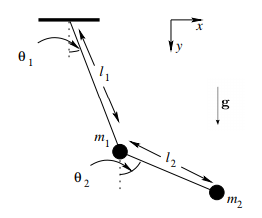
\includegraphics[width=175px]{doublepend.PNG}
\caption{A simple gravity double pendulum (model assumes no friction or air
resistance)[1]}
	\label{fig:maxresdefault}
\end{figure}

\subsection{Table of Units}

Throughout this document SI (Syst\`{e}me International d'Unit\'{e}s) is
employedas the unit system. In addition to the basic units, several derived
units are
used as described below.  For each unit, the symbol is given followed by a
description of the unit and the SI name.\\

\renewcommand{\arraystretch}{1.2}
\begin{center}
  \noindent \begin{tabular}{l l l} 
    \toprule		
    \textbf{symbol} & \textbf{unit} & \textbf{SI}\\
    \midrule 
    \si{\metre} & length & metre\\
    \si{\kilogram} & mass & kilogram\\
    \si{\second} & time & second\\
    \bottomrule
  \end{tabular}
\end{center}

\newpage

\subsection{Table of Symbols}

The table that follows summarizes the symbols used in this document along with
their units. The choice of symbols was made to be consistent with calculus,
ordinary
differentials (ODE), the Lagrangian, kinematics etc. The standard mathematical
spaces
are used (e.g. $\mathbb{N}$, $\mathbb{Z}$, $\mathbb{R}$, etc.) as well as some 
additional spaces defined in the following table. 
~\newline
\renewcommand{\arraystretch}{1.2}
\noindent \begin{longtable*}{l l l p{8cm}} \toprule
\textbf{symbol} & \textbf{space} & \textbf{unit} & \textbf{description}\\
\midrule 
$g$ & $\mathbb{R}$ & -- & gravitational constant
\\
$m_1$ & $\mathbb{R}$ & -- & mass of the 1st pendulum weight
\\ 
$m_2$ & $\mathbb{R}$ & -- & mass of the 2nd pendulum weight
\\ 
$m_n$ & $\mathbb{R}$ & -- & mass of the nth pendulum weight
\\ 
$l_1$ & $\mathbb{R}$ & -- & length of the 1st pendulum rod
\\ 
$l_2$ & $\mathbb{R}$ & -- & length of the 2nd pendulum rod
\\ 
$l_n$ & $\mathbb{R}$ & -- & length of the nth pendulum rod
\\
$\theta_1$ & $\mathbb{R}$ & -- & amplitude from the pivot point
\\
$\theta_2$ & $\mathbb{R}$ & -- & amplitude from the 1st pendulum weight
\\
$\theta_n$ & $\mathbb{R}$ & -- & amplitude from the nth pendulum weight
\\
$L$ & $\sum\mathbb{R}$ & -- & Pendulum system Lagrangian
\\
$T$ & $\sum\mathbb{R}$ & -- & Kinetic energy of system
\\
$V$ & $\sum\mathbb{R}$ & -- & Potential energy of system
\\
$P(x)$ & $\mathbb{Z} \times \mathbb{R} \implies \mathbb{R}$ & -- & Poincaré map P projects point x onto point P(x)
\\
\bottomrule
\end{longtable*}

\newpage
\subsection{Abbreviations and Acronyms}

The symbols are listed in alphabetical order.\\

\renewcommand{\arraystretch}{1.2}
\begin{tabular}{l l} 
  \toprule		
  \textbf{symbol} & \textbf{description}\\
  \midrule 
  A & Assumption\\
  DD & Data Definition\\
  GD & General Definition\\
  GS & Goal Statement\\
  IM & Instance Model\\
  LC & Likely Change\\
  NF & Non-Functional Requirement\\
  PS & Physical System Description\\
  R & Requirement\\
  SRS & Software Requirements Specification\\
  T & Theoretical Model\\
  \bottomrule
\end{tabular}\\

\newpage

\pagenumbering{arabic}

\setcounter{secnumdepth}{3}

\section{Introduction}

This documents is an SRS for the \progname program. The directory for this
project can
be found at GitHub:
\href{https://github.com/karolserkis/CAS-741-Pendula/}{/karolserkis/CAS-741-Pendula/}

\subsection{Purpose of Document}
The purpose of this document is to describe the requirements for a
\progname program solution that
only focuses on multi-pendulum simulations (double \& triple pendula and beyond)and tracking the chaotic
motion of the system. It will allow users to generate diagrams (e.g. Poincare
mapping)
and plot trajectories over time using two different ODE/DAE initial value
problem solvers. In the case of
a double pendulum you have a new system that is dynamic and chaotic and
requires a set of coupled ordinary differential equation solvers. Once one
introduces
multiple
pendula the system becomes chaotic and interesting to model and simulate. 

The theoretical models used in the \progname code will be provided, insuring
assumptions and unambiguous definitions are identified. This document 
is intended to be used as a reference to provide all information necessary to 
understand and verify the inputs to outputs. The SRS is abstract: the contents 
describe the problem being solved, but not how to solve it.

This document will be used as a starting point for subsequent development
phases, including writing the design specification and the software
verification and validation plan. The verification and validation plan will show
the steps inthe software documentation/implementation.

\subsection{Scope of Requirements} 

The scope of the \progname program is limited to the generation 
of diagrams and plot trajectories that are possible to run and compute on a
local system.

Assumptions: The \progname will be a closed system. Air resistance and friction
will
not be considered for the simulation. The \progname will be limited to the user
initialized inputs and
the output of the \progname will either plot trajectories over time, generate
diagrams, like Poincare mapping
and limit the user to a specific duration of the simulation, in order to allow
diagrams and trajectory history to be saved.
The user will be able to set a range of time and initialize the system. \\

\subsection{Characteristics of Intended Reader} 
Simplification of some physical concepts are proposed to make the document
technically accessible and also the software to be accessible.
Nevertheless, the intended reader is expected to have a basic knowledge in
mathematics (calculus, differentials/ODEs) and physics (kinematics, energy
potential, Lagrangian, Poincare mapping) is recommended to get a deeper
understanding of the document.

\subsection{Organization of Document}
\begin{itemize}
\item The organization of this document follows the template for an SRS for
scientific
computing software proposed by Dr. Spencer Smith. 
\item The presentation follows the standard pattern of presenting goals,
theories, definitions, and assumptions.
\item The goal statements are refined to the theoretical models, and the
theoretical
models to the instance models. The data definitions are used to support the
definitions of the different models.
\end{itemize}
\newpage
\section{General System Description}
This section identifies the interfaces between the system and its environment,
describes the user characteristics and lists the system constraints.

\subsection{System Context}

\begin{center}
\framebox{\textbf {USER}} $ \xLongleftrightarrow[\textbf{Input with the
User}]{\textbf{User enters input}} $\framebox{\textbf { \progname}}
$ \xLongleftrightarrow[\textbf{Output to the User}] {\textbf{User sees results}}$\framebox{\textbf {USER}}\\
\end{center}

\begin{itemize}
\item User Responsibilities:
\begin{itemize}
\item Ensure that the input data is fits the system model.
\item Ensure that the input data is within scope.
\end{itemize}
\item \progname program Responsibilities:
\begin{itemize}
\item Detect data type mismatch, such as a string of characters instead of a
  floating point number.
\item Determine if the inputs satisfy the required physical and software 
  constraints.
\item Solve the system of equations arising from the input data to generate 
  the output data.
\item Generate a plot of the output data and generate diagrams to display to the user.
\end{itemize}
\end{itemize}

\subsection{User Characteristics}
The end user of \progname program should have an understanding of first year 
undergraduate math and physics. Less understanding of physics and math are
required to use the software than understand
this document or the inner workings of the software program.

\subsection{System Constraints}
There are no system constraints. The \progname software will be created with
multi-platform support.

\newpage
\section{Specific System Description}

This section first presents the problem description, which gives a high-level
view of the problems to be solved and the motivation behind \progname software.
This is followed by the solution
characteristics specification, which presents the assumptions, theories, 
definitions and finally the instance models.

\subsection{Problem Description}

The \progname software will generate a plot trajectory in a 3D plot grid.
A simple gravity pendulum has very easy to system to model and consists of a
weight suspended from a pivot and the weight is given enough space to swing
freely. To simplify the model we assume no air resistance with a frictionless
pivot. The model and calculations for the simple gravity pendulum are well
defined and only require simple derivations and differential solvers.

\progname program will produce a simulation given a set of equilibrium constantsand input.
Terminologies and the physical system are described below.

\subsubsection{Terminology and Definitions}

This subsection provides a list of terms that are used in the subsequent
sections and their meaning, with the purpose of reducing ambiguity and making
it easier to correctly understand the requirements:

\begin{description}
\item[Equilibrium position:] The pendulum rod and weight position in its resting state.
\item[3D Cartesian coordinate system:] The pendulum rod and weight swing from a
pivot position origin $(x,y,z)$
\end{description}

\begin{figure}[H]
	\centering
	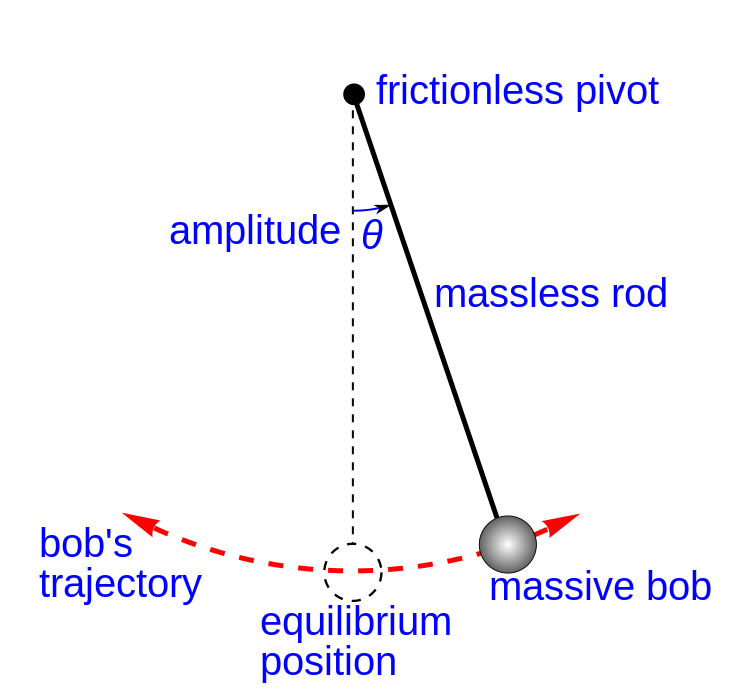
\includegraphics[width=190px]{simple-pend.png}
\caption{A simple gravity pendulum where the model assumes no friction or air
resistance}
	\label{fig:maxresdefault}
\end{figure}

\begin{description}
\item[Lagrangian:] The $L=T-V$, where T and V are the kinetic and potential
energies of the system respectively.
\item[Poincaré map:] Starting with the poincaré section of the \progname in 3D space, the poincaré map P
is a projection from point x onto point P(x) transforming the 3D space into a 2D projection diagram plot.
\end{description}

\subsubsection{Physical System Description}

The physical system of \progname program includes the following elements:

\begin{itemize}
\item[PS1:] Simulate an n-rod multi-pendulum system with no friction and no air
resistance in a 3D space.
\end{itemize}

\begin{figure}[H]
	\centering
	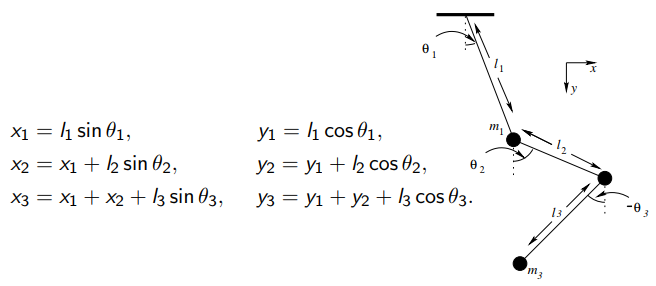
\includegraphics[width=450px]{triplependula.PNG}
\caption{A triple pendulum example[1]}
	\label{fig:maxresdefault}
\end{figure}

\subsubsection{Goal Statements}

\noindent Given the user input and the initial state of the \progname with reference to the table of symbols the goal
statements are:

\begin{itemize}

\item[GS\refstepcounter{goalnum}\thegoalnum:] Generate a trajectory plot and a poincaré map plot of 
the movement of the pendula from equilibrium state of rest and show logged
statistics over time to the user.
\end{itemize}


\newpage

\subsection{Solution Characteristics Specification}

\subsubsection{Assumptions}

This section simplifies the original problem and helps in developing the
theoretical model by filling in the missing information for the physical
system. The numbers given in the square brackets refer to the theoretical model
[T], general definition [GD], data definition [DD], instance model [IM], or
likely change [LC], in which the respective assumption is used.

\begin{itemize}
\item[A\refstepcounter{assumpnum}\theassumpnum:]
  All generated simulation diagrams will fit the mathematical model and scope.
\item[A\refstepcounter{assumpnum}\theassumpnum:]
The user knows what the purpose of the simulation model and inputs weights and lengths
according to possible simulation characteristics.
\item[A\refstepcounter{assumpnum}\theassumpnum:]
In the model we assume no air resistance with a frictionless pivot.
\end{itemize}

\newpage

\subsubsection{Theoretical Models}\label{sec_theoretical}

This section focuses on the general equations and laws that \progname program is based
on.\\

\noindent
\begin{minipage}{\textwidth}
\renewcommand*{\arraystretch}{1.5}
\tabulinesep=1.5mm
\begin{tabu}{| p{\colAwidth} | p{\colBwidth}|}
  \hline
  \rowcolor[gray]{0.9}
  Number& T\refstepcounter{theorynum}\thetheorynum\\
  \hline
  Label&\bf Double Pendulum Pivot rod \\
  \hline
  Equation&  
$$x_1 = l_1 \sin\theta_1 \quad\quad y_1 = -l_1 \cos\theta_1$$
$$x_2 = l_1 \sin\theta_1 + l_2 \sin\theta_2 \quad\quad y_2 = -l_1\cos\theta_1
-l_2\cos\theta_2$$\\
  \hline
  Description & Simple coordinate model system solution\\
  \hline
  Source & [6]\\
  \hline
  Ref.\ By &--\\
  \hline
\end{tabu}
\end{minipage}\\

\noindent
\begin{minipage}{\textwidth}
\renewcommand*{\arraystretch}{1.5}
\tabulinesep=1.5mm
\begin{tabu}{| p{\colAwidth} | p{\colBwidth}|}
  \hline
  \rowcolor[gray]{0.9}
  Number& T\refstepcounter{theorynum}\thetheorynum\\
  \hline
  Label&\bf Double Pendulum Potential Energy\\
  \hline
  Equation&  
$$ T = \displaystyle\frac{1}{2}m_1v_1^2 + \frac{1}{2}m_2v_2^2 $$
$$ = \frac{1}{2}m_1(\dot{x}_1^2 + \dot{y}_1^2) + \frac{1}{2}m_2(\dot{x}_2^2 +
\dot{y}_2^2) $$
$$ = \frac{1}{2}m_1 l_1^2 \dot{\theta}_1^2 + \frac{1}{2}m_2\left[l_1^2
\dot{\theta}_1^2 + l_2^2 \dot{\theta}_2^2 + 2l_1l_2\dot{\theta}_1\dot{\theta}_2
\cos(\theta_1 - \theta_2)\right]$$\\
  \hline
  Description & Potential Energy model system solution\\
  \hline
  Source & [6]\\
  \hline
  Ref.\ By &--\\
  \hline
\end{tabu}
\end{minipage}\\


\noindent
\begin{minipage}{\textwidth}
\renewcommand*{\arraystretch}{1.5}
\tabulinesep=1.5mm
\begin{tabu}{| p{\colAwidth} | p{\colBwidth}|}
  \hline
  \rowcolor[gray]{0.9}
  Number& T\refstepcounter{theorynum}\thetheorynum\\
  \hline
  Label&\bf Double Pendulum Potential Energy\\
  \hline
  Equation&  
$$V = m_1 g y_1 + m_2gy_2$$
$$= -m_1 g l_1 \cos\theta_1 - m_2 g (l_1 \cos\theta_1 + l_2 \cos\theta_2)$$
$$= -(m_1 + m_2) g l_1 \cos\theta_1 - m_2 g l_2\cos\theta_2$$\\
  \hline
  Description & Potential Energy model system solution\\
  \hline
  Source & [6]\\
  \hline
  Ref.\ By &--\\
  \hline
\end{tabu}
\end{minipage}\\

\noindent
\begin{minipage}{\textwidth}
\renewcommand*{\arraystretch}{1.5}
\tabulinesep=1.5mm
\begin{tabu}{| p{\colAwidth} | p{\colBwidth}|}
  \hline
  \rowcolor[gray]{0.9}
  Number& T\refstepcounter{theorynum}\thetheorynum\\
  \hline
  Label&\bf Double Pendulum Lagrangian ($L=T-V$)\\
  \hline
  Equation&  
$$L =\frac{1}{2}(m_1 + m_2) l_1^2 \dot{\theta}_1^2 + \frac{1}{2}m_2 l_2^2
\dot{\theta}_2^2 + m_2l_1l_2\dot{\theta}_1\dot{\theta}_2 \cos(\theta_1 -
\theta_2)$$
    $$+ (m_1 + m_2) g l_1 \cos\theta_1 + m_2 g l_2\cos\theta_2$$\\
  \hline
  Description & Lagrangian model system solution\\
  \hline
  Source & [6]\\
  \hline
  Ref.\ By &--\\
  \hline
\end{tabu}
\end{minipage}\\

\noindent
\begin{minipage}{\textwidth}
\renewcommand*{\arraystretch}{1.5}
\tabulinesep=1.5mm
\begin{tabu}{| p{\colAwidth} | p{\colBwidth}|}
  \hline
  \rowcolor[gray]{0.9}
  Number& T\refstepcounter{theorynum}\thetheorynum\\
  \hline
  Label&\bf Poincaré map($P(x)$)\\
  \hline
  Equation&  
$$P(x) :\mathbb{Z} \times \mathbb{R} \implies \mathbb{R}$$\\
  \hline
  Description & Poincaré map P projects point x onto point P(x)\\
  \hline
  Source & [6]\\
  \hline
  Ref.\ By &--\\
  \hline
\end{tabu}
\end{minipage}\\


\subsubsection{General Definitions}\label{sec_gendef}

We will use the Lagrangian and ODEs. No need for general definitions in
current documentation.

\subsubsection{Data Definitions}\label{sec_datadef}

This section collects and defines all the data needed to build the instance
models. The models here are to satisfy the theoretical models constrained and closed 3D space.\\

\noindent
\begin{minipage}{\textwidth}
\renewcommand*{\arraystretch}{1.5}
\tabulinesep=1.5mm
\begin{tabu}{| p{\colAwidth} | p{\colBwidth}|}
  \hline
  \rowcolor[gray]{0.9}
  Label&\bf Closed, Real intervals\\
  \hline
  Equation&  
$$\mathbb{R} (\texttt{for Langrangian equation})$$
$$ P(x) :\mathbb{Z} \times \mathbb{R} \implies \mathbb{R}$$\\
  \hline
  Description & Simple cartesian coordinate model system solution\\
  \hline
  Source & [6]\\
  \hline
  Ref.\ By & T1,T2,T3,T4,T5\\
  \hline
\end{tabu}
\end{minipage}\\

\subsubsection{Instance Models} \label{sec_instance}    

This section transforms the problem defined in problem description into 
one which is expressed in mathematical terms. \\

\noindent
\begin{minipage}{\textwidth}
\renewcommand*{\arraystretch}{1.5}
\tabulinesep=1.5mm
\begin{tabu}{| p{\colAwidth} | p{\colBwidth}|}
  \hline
  \rowcolor[gray]{0.9}
  Label&\bf Addition of closed, real intervals\\
  \hline
  Equation&  
$$\sum \mathbb{R} (\texttt{for Langrangian equation})$$
$$ P(x) :\mathbb{Z} \times \mathbb{R} \implies \mathbb{R}$$\\
  \hline
  Description & Simple cartesian coordinate model system solution\\
  \hline
  Source & [6]\\
  \hline
  Ref.\ By & T1,T2,T3,T4,T5\\
  \hline
\end{tabu}
\end{minipage}\\

\subsubsection{Data Constraints} \label{sec_DataConstraints}    

The data constraints on the input and output variables, respectively.  
The column for physical constraints gives the physical limitations on 
the range of values that can be taken by the
variable.  The column for software constraints restricts the range of inputs to
reasonable values.  The constraints are conservative, to give the user of the
model the flexibility to experiment with unusual situations.  The column of
typical values is intended to provide a feel for a common scenario.  The
uncertainty column provides an estimate of the confidence with which the
physical quantities can be measured.  This information would be part of the
input if one were performing an uncertainty quantification exercise.

\begin{itemize}
\item Constraint on gravity: g = $9.8 m/s^2$
\end{itemize}

\subsubsection{Properties of a Correct Solution}

\noindent
A correct solution must satisfy the system of non-linear equations described. 
The user will also be able to judge the results based on the knowledge about the model and input.

\newpage
\section{Requirements}

This section provides the functional requirements, the business tasks that the
software is expected to complete, and the nonfunctional requirements, the
qualities that the software is expected to exhibit.


\subsection{Functional Requirements}

\noindent \begin{itemize}

\item[R\refstepcounter{reqnum}\thereqnum:] \progname program will 
  take the following inputs:
  \begin{enumerate} \item The initial mass of the weights. 
                    \item The inital length of the rods.
  \end{enumerate}

\item[R\refstepcounter{reqnum}\thereqnum:] \progname program
will ensure that the inputs do not violate the constraints specified in the Data Contraints section:
    \begin{enumerate} \item \progname program will 
generate diagrams with and plot lines and timeline of logged movement. 
\item The timeline of swings of the pendulum will be logged and eventually
return to a resting state in equilibrium
\end{enumerate}

\item[R\refstepcounter{reqnum}\thereqnum:] \progname program will 
  take the following inputs:
  \begin{enumerate} \item The initial mass of the weights. 
                    \item The inital length of the rods.
  \end{enumerate}

\end{itemize}
\newpage
\subsection{Nonfunctional Requirements}

\progname program will be try to be small and simple, so performance is not a 
priority. Any reasonable implementation will be very quick and use minimal 
storage. Rather than performance, the non-functional requirement priorities 
are correctness, understandability, reusability, maintainability, and 
portability. 

\begin{itemize}
\item[NF\refstepcounter{nfreqnum}\thenfreqnum:] \progname program access axis
labels \& 3D cartesian coordinates.
\end{itemize}

\subsubsection*{Correctness}
\begin{itemize}
	\item The \progname tool must be correct in its generation of plot trajectories.
\end{itemize}

\subsubsection*{Reliability}

The \progname should run successfully on all platforms.

\subsubsection*{Robustness}
\begin{itemize}
	\item The \progname must be able to recognize violated data 
	constraints and report them to the user.
	\item The \progname tool must inform the user when it encounters any 
	unspecified state.
\end{itemize}

\subsubsection*{Performance}
Performance is a priority in the \progname
specification. It needs to be able to generate a plot reasonable amount of time.

\subsubsection*{Verifiability}
\begin{itemize}
	\item The \progname must be verifiable with respect to the 
	correctness of its calculations. The calculation 
	procedures used by the \progname tool must be implemented such that 
	they can be verified using mathematical proofs.
\end{itemize}

\subsubsection*{Usability}
\begin{itemize}
	\item The user must be able to enter values using standard mathematical 
	notation.

	\item The plot should generate and be large enough for the user's display.
\end{itemize}

\subsubsection*{Maintainability}
\begin{itemize}
	\item The evolvability of the \progname must allow the addition 
	of real intervals.
\end{itemize}

\subsubsection*{Reusability}
Reusability is not a priority because there are currently no future products 
that will rely on \progname

\subsubsection*{Portability}
The portability of the \progname will be multi-platform.

\newpage

\section{Likely Changes}    

\noindent \begin{itemize}

\item[LC\refstepcounter{lcnum}\thelcnum:] Generation of diagrams 
  using distributed/parallel computing

\end{itemize}

\subsection*{References}\label{ssec:ref}
\begin{itemize}
\item{[1]} Dynamics of multiple pendula \\\url{http://wmii.uwm.edu.pl/~doliwa/IS-2012/Szuminski-2012-Olsztyn.pdf}
\item{[2]} Pendulum \\\url{https://en.wikipedia.org/wiki/Pendulum}
\item{[3]} Pendulum (mathematics)
\\\url{https://en.wikipedia.org/wiki/Pendulum_(mathematics)}
\item{[4]} Double Pendulum
\\\url{https://en.wikipedia.org/wiki/Double_pendulum}\item{[4]}
Differential-Algebraic Equations by Taylor Series
\\\url{http://www.cas.mcmaster.ca/~nedialk/daets/}
\item{[5]} Multi-body Lagrangian Simulations
\\\url{https://www.youtube.com/channel/UCCuLchOx0W0yoNE9KOCYlVQ}
\item{[6]} The double pendulum: Lagrangian formulation
\\\url{https://diego.assencio.com/?index=1500c66ae7ab27bb0106467c68feebc6}
\item{[7]} Poincaré map
\\\url{https://en.wikipedia.org/wiki/Poincar%C3%A9_map}
\end{itemize}

\bibliographystyle {plainnat}
\bibliography {../../ReferenceMaterial/SRS_Refs}

\end{document}